%!TEX TS-program = xelatex
%!TEX encoding = UTF-8 Unicode

%%%  Syllabus template for use with style files at http://kjhealy.github.com/latex-custom-kjh
%%%  Kieran Healy

\documentclass[11pt,article,oneside]{memoir}

% packages
\usepackage{org-preamble-xelatex}
\usepackage{wallpaper}
\usepackage{xcolor}
\usepackage{enumitem}
\usepackage{multicol}
\setlength{\columnsep}{1em}
\usepackage{booktabs}
\newcommand{\ra}[1]{\renewcommand{\arraystretch}{#1}}

\AtBeginBibliography{\small}

% Definitions
\def\myauthor{Author}
\def\mytitle{Title}
\def\mycopyright{\myauthor}
\def\mykeywords{}
\def\mybibliostyle{plain}
\def\mybibliocommand{}
\def\mysubtitle{}
\def\myaffiliation{Louisiana State University}
\def\myaddress{309 Design}
\def\myemail{baharmon@lsu.edu} 
\def\myweb{https://baharmon.github.io/}
\def\myphone{919.622.8414}
\def\myversion{}
\def\myrevision{}
\def\myaffiliation{\ \\Louisiana State University}
\def\myauthor{Brendan Harmon}
\def\mykeywords{Landscape Architecture, Syllabus}
\def\mytitle{{\normalsize LA 7051 | {\sffamily\mdseries Advanced Topics Studio} \newline} \Large \bfseries Computational Ecology} 
\def\mysubtitle{\sffamily\mdseries {\normalsize Yosemite National Park}}

% color
\makeatletter
\newcommand{\globalcolor}[1]{%
  \color{#1}\global\let\default@color\current@color
}
\makeatother

% begin
\begin{document}

\setlength\bibitemsep{0.75em}

% fonts
\defaultfontfeatures{}
\defaultfontfeatures{Scale=MatchLowercase}         
\setmainfont[Scale=1, Path = fonts/lato/,BoldItalicFont=Lato-RegIta,BoldFont=Lato-Reg,ItalicFont=Lato-LigIta]{Lato-Lig}
\setsansfont[Scale=1, Path = fonts/lato/,BoldItalicFont=Lato-RegIta,BoldFont=Lato-Reg,ItalicFont=Lato-LigIta]{Lato-Lig}
\setmonofont[Mapping=tex-text,Scale=0.8,Path = fonts/inconsolata/]{i}

\def\ind{\hangindent=1 true cm\hangafter=1 \noindent}
\def\labelitemi{$\cdot$}
\chapterstyle{article-4-sans}  
\title{\LARGE \mytitle \newline \mysubtitle}     
\author{\large\myauthor \newline \footnotesize\texttt{\noindent\myemail}}
\date{\normalsize Fall 2018. Design 217.\newline Monday, Wednesday, \& Friday \newline 1:30pm--5:30pm.}
\published{\,}

% -------------------------------- COVER PAGE -------------------------------- 

\pagenumbering{gobble}
\globalcolor{black}
\vspace*{-10em}
\maketitle
\ThisCenterWallPaper{1}{../images/yosemite/yosemite_portrait_2.png}
\vfill
\clearpage

% -------------------------------- DESCRIPTION -------------------------------- 

\pagenumbering{arabic}
\globalcolor{black}
\vspace*{-10em}
\maketitle

\section{Course description}
In this studio you will learn computational methods for ecological modeling
and use them to plan for the future of Yosemite national park. 
This studio will introduce advanced topics in landscape ecology and biodiversity conservation
such as shifting ecological baselines, process-form interaction, 
systematic conservation planning, and climate change adaptation. 
You will learn how to model ecological patterns and simulate ecological processes
using Geographic Information Systems (GIS). 
You will learn visual programming, geospatial programming in Python, 
digital fabrication methods, and advanced 3D rendering. 
You will apply these methods to develop a long-term landscape plan
for the national park. 
Each week you will spend 
a day in a seminar discussing ecological theory and its applications,
a day in a workshop learning new computational methods,
and a day developing your projects.
%

\section{Optional fieldtrip}
There will be an optional fieldtrip to Yosemite National Park
the week before the semester starts. 
% Estimated cost: $750

%\clearpage

% -------------------------------- SCHEDULE -------------------------------- 

\section{Course schedule}
\small
%
\begin{multicols}{3}
\begin{enumerate}[label=\textbf{\arabic*}]
%
\item Landscape ecology
\item Programming
\item Form \& process
\item Baselines
\item Suitability
\item Viewsheds
\item Corridors
\item Land change
\item Fire simulation
\item Flood simulation
\item Digital fabrication
\item Planning I
\item Planning II
\item 3D rendering
\item Final review
%
\end{enumerate}
\end{multicols}

\clearpage

% -------------------------------- FIGURES -------------------------------- 

%\begin{figure}
%\begin{center}
%%
%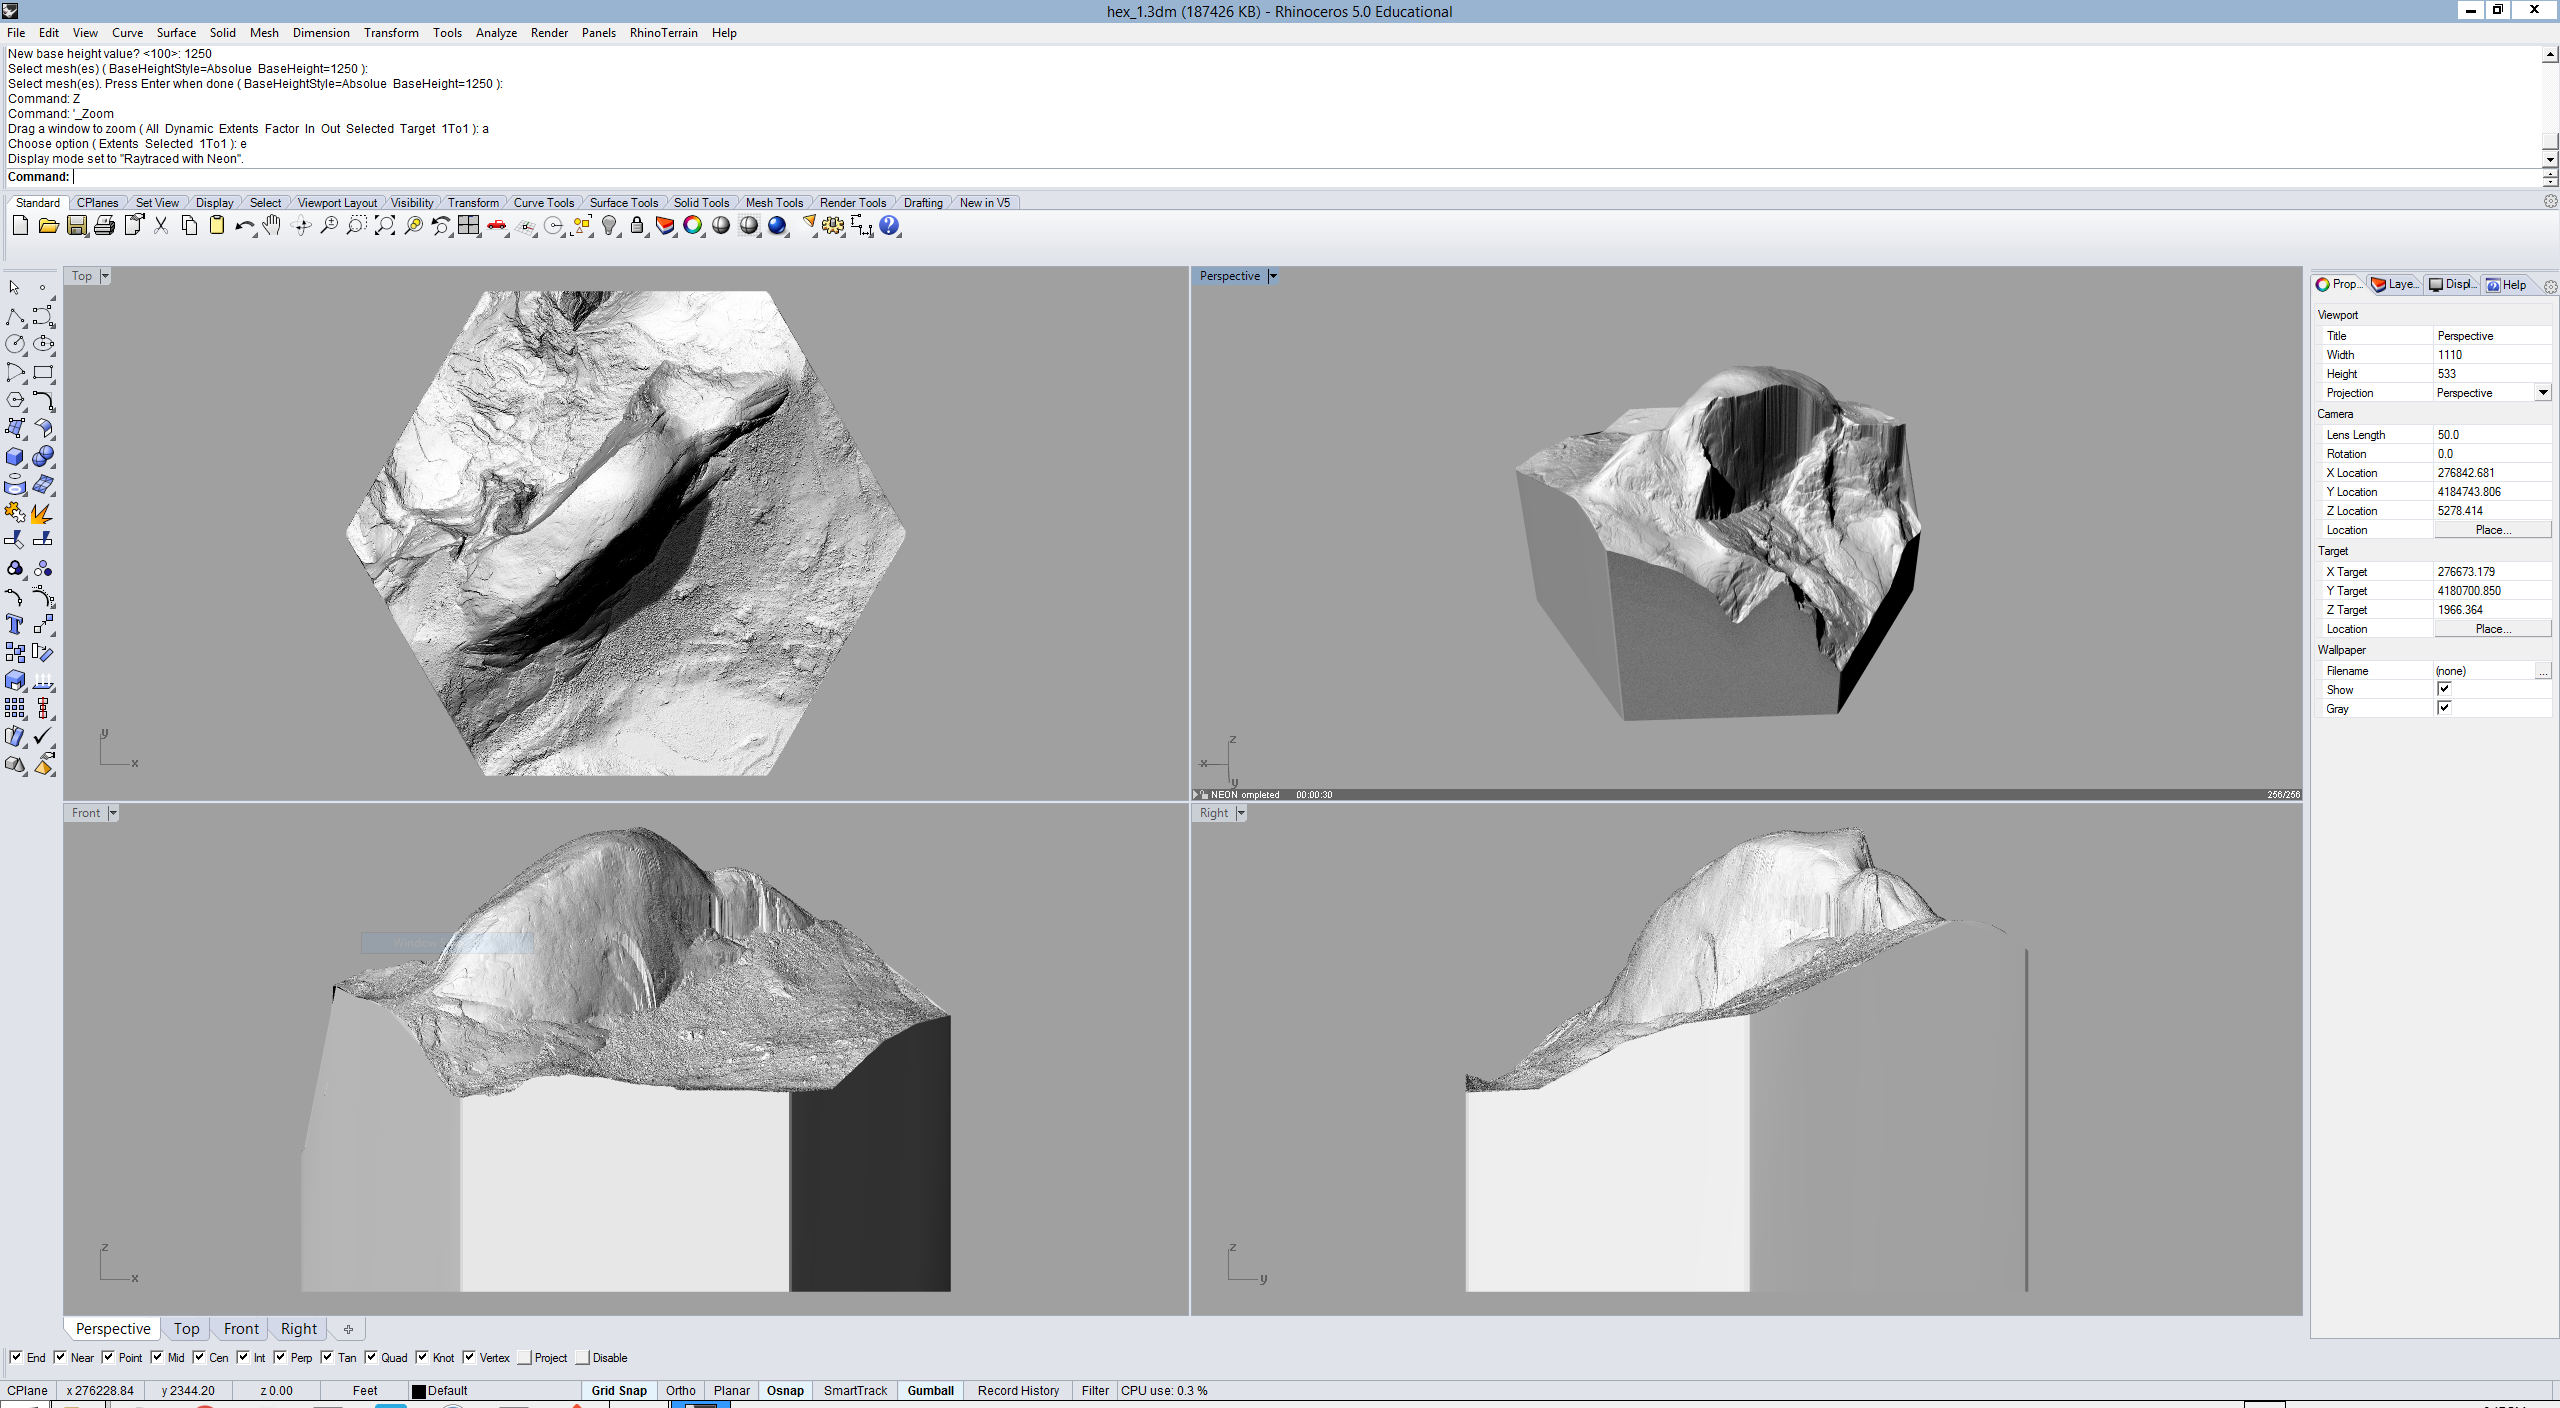
\includegraphics[height=4.4cm]{../images/yosemite/half_dome_hex_with_base.png} \hspace{0.25cm}
%%
%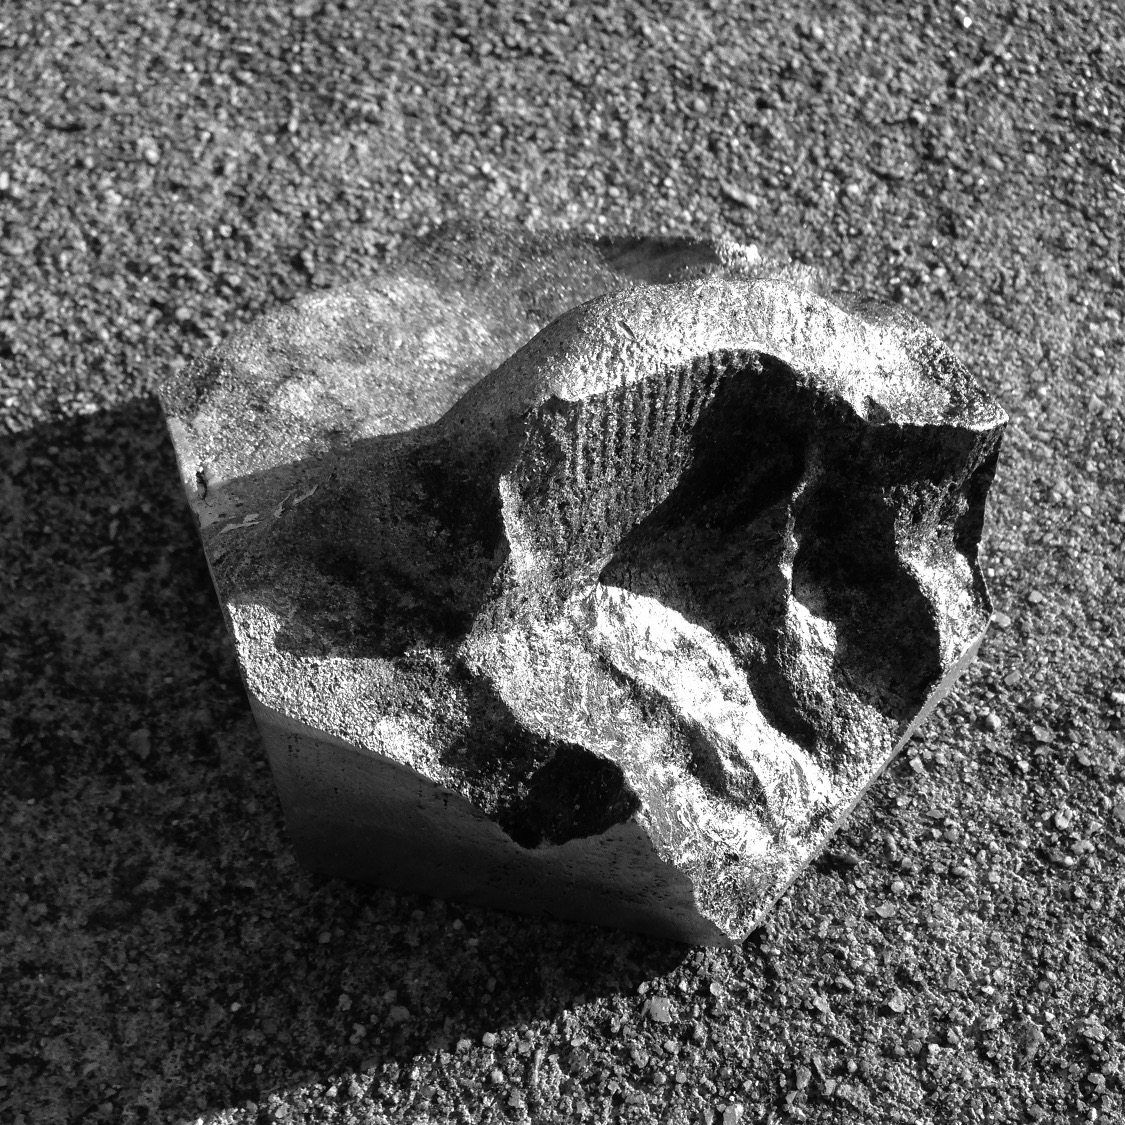
\includegraphics[height=4.4cm]{../images/yosemite/half_dome_sq_greyscale.jpg}
%\caption{3D model and cast aluminum model of Half Dome, Yosemite}
%%
%\label{fig:unbuilt_houses}
%\end{center}
%\end{figure}

%\clearpage

% -------------------------------- PROJECTS -------------------------------- 
\section{Projects}
\normalsize
At the final review you will present your work from all three projects -- 
mapping and analysis, landscape planning, and reserve design -- 
in an engaging narrative that explains the challenges faced by the park, 
your landscape planning methodology, and your design. 
\\

\noindent \textbf{Mapping \& analysis}
You will develop a series of maps and other media that describe the national park,
its physical environment, and ecological patterns and processes. 
Your work should introduce the biodiversity conservation issues 
faced by the park.
Deliverables may include maps, renderings, animations, video, and text. 
% The review will be floating, gallery style. Pin up the evening before.
\textbf{Due:} week 5.
\\

\noindent \textbf{Planning methodology}
You will develop a landscape planning methodology 
for developing a long-term master plan for the national park. 
Begin with a suitability analysis using map overlays
You should should also develop graphics that explain your planning methodology. 
% The review will be floating, gallery style. Pin up the evening before.
\textbf{Due:} week 10.
\\

\noindent \textbf{Landscape planning}
You will design a long-term masterplan for the national park
that addresses contemporary and emerging ecological issues. 
Your masterplan should evolve over time, 
address multiple spatial and temporal scales, 
engage visitors in the park's ecological processes,
and aesthetically express the uniqueness and dynamism of the landscape. 
Deliverables include an illustrative masterplan, a CNC milled terrain model, 
phasing diagrams, diagrams illustrating management regimes, and 3D renderings.
\textbf{Due:} week 15.
\\

% -------------------------------- Grading -------------------------------- 
\section{Grading}

\begin{table}[H]
\small
\begin{tabular}{l l l l l l}
\textbf{Mapping} & 25\% &
\textbf{Methodology} & 25\% &
\textbf{Planning} & 50\% \\
\end{tabular}
\end{table}

% -------------------------------- Software -------------------------------- 
\section{Software}
GRASS GIS | \url{https://grass.osgeo.org/}\\
Blender | \url{https://www.blender.org/}\\
Rhinoceros | \url{https://www.rhino3d.com/}\\
RhinoTerrain | \url{http://www.rhinoterrain.com/}\\
RhinoCAM | \url{https://mecsoft.com/rhinocam-software/}\\

\clearpage

% -------------------------------- TOPICS -------------------------------- 
\section{Topics}
\normalsize

\noindent \textbf{Landscape ecology}
An introduction to landscape ecology and biodiversity conservation.
The methods workshop will cover 
ecological census techniques, interpolation methods, and
hotspot analysis. 
%
\nocite{*} \printbibliography[keyword=intro, heading=none]
\vspace*{0.5em}
% readings: ecological census techniques, priortizing conservation with hotspots

\noindent \textbf{Geospatial programming}
A series of methods workshop will introduce visual programming, python programming, and python scripting in GIS. 
You will also learn how to use Git, a version control system, to maintain your code.
%
\nocite{*} \printbibliography[keyword=python, heading=none]
\vspace*{0.5em}

\noindent \textbf{Form \& process}
%  <---------------------------------------------------EDITING HERE
%
\nocite{*} \printbibliography[keyword=form_and_process, heading=none]
\vspace*{0.5em}
% readings: ...

%Seminar: form and process
%Methods lecture: flooding, water flow, erosion
%Methods walkthrough: r.geomorphons, r.watershed, r.stream*, r.lake, rulse3D, avalanche



\noindent \textbf{Ecological baselines}
...  % climate change
%
\nocite{*} \printbibliography[keyword=form_and_process, heading=none]
\vspace*{0.5em}
% readings: rewilding, shifting baselines, long term eco, alternative futures for willamete valley

%Seminar: baselines, rewilding, and restoration
%Methods lecture: landfire data, ...

% Donlan, Rewilding North America
%R. Corlett, The Role of Rewilding in Landscape Design for Conservation, 
%P. Martin, Twilight of the Mammoths: Ice Age Extinctions and the Rewilding of America
%J. Donlan, Re-wilding North America. Rubenstein DR, 
%D.I. Rubenstein, Pleistocene Park: Does re-wilding North America represent sound conservation for the 21st century?
%W. Cornwall, Have returning wolves really saved Yellowstone? 


\noindent \textbf{Suitability analysis}
... 
%
\nocite{*} \printbibliography[keyword=suitability, heading=none]
\vspace*{0.5em}
% readings: design with nature, systematic conservation planning

%Seminar: habitat identification, patches, richness, and overlay analysis
%Topics: Ian McHarg, systematic conservation planning, & alternative futures
%Methods lecture: classification, summary statistics, overlay analysis
%Methods walkthrough: image segmentation and classification, v.habitat.dem, r.watershed, r.stream*, r.stats, & r.series


\noindent \textbf{Viewsheds}
...  % Viewshed
%
\nocite{*} \printbibliography[keyword=viewsheds, heading=none]
\vspace*{0.5em}
% readings: ...

%  r.viewshed.cva, PCA, skyiew


\noindent \textbf{Corridors}
... % migration and climate change adaption
%
\nocite{*} \printbibliography[keyword=corridors, heading=none]
\vspace*{0.5em}
% readings: land mosaics, sloss, sloss debate, theory of  island biogeography

%Seminar: fragmentation, connectivity, and corridor design
%Topics: SLOSS, migration routes, & climate refugees
%Methods lecture: landscape structure, overlay analysis, least cost path analysis, & r.connectivity*
%Methods walkthrough: r.li, r.mapcalc, r.cost, r.drain, r.walk, &  v.net.salesman




\noindent \textbf{Land change}
... 
%
\nocite{*} \printbibliography[keyword=futures, heading=none]
\vspace*{0.5em}
% readings: futures

%Seminar: ecological succession, flooding, urban growth, and land change
%Methods lecture: land change modeling
%Methods walkthrough: r.futures.* & ITZI


\noindent \textbf{Fire simulation}
... 
%
\nocite{*} \printbibliography[keyword=fire, heading=none]
\vspace*{0.5em}
% readings: tl chapter, fire disturbance regimes?

\noindent \textbf{Flood simulation}
... 
%
\nocite{*} \printbibliography[keyword=flooding, heading=none]
\vspace*{0.5em}
% readings: ...

\noindent \textbf{Digital fabrication}
... 
%
\nocite{*} \printbibliography[keyword=fabrication, heading=none]
\vspace*{0.5em}
% readings: ...

\noindent \textbf{Landscape planning}
... 
%
\nocite{*} \printbibliography[keyword=planning, heading=none]
\vspace*{0.5em}
% readings: ...

\noindent \textbf{3D rendering}
... % Python scripting
%
\nocite{*} \printbibliography[keyword=viz, heading=none]
\vspace*{0.5em}
% readings: TL book and papers, blender tutorials, geo modeling website

\clearpage

% -------------------------------- Readings -------------------------------- 
\section{Readings}
\renewcommand*{\bibfont}{\normalsize} %\small
\vspace*{0.5cm}
\nocite{*}
\setlength\bibitemsep{1\baselineskip}
\printbibliography[heading=none]

\clearpage

% -------------------------------- Policies -------------------------------- 
\section{Policies}

\noindent \textbf{Time Commitment Expectations}
LSU's general policy states that for each credit hour, you (the student) should plan to
spend at least two hours working on course related activities outside of class. Since this course is for six credit hours, you should expect to spend a minimum of twelve hours outside of class each week working on assignments for this course. For more information see: 
\url{http://catalog.lsu.edu/content.php?catoid=12&navoid=822}.\\

\noindent \textbf{LSU student code of conduct}
The LSU student code of conduct explains student rights, excused absences, and what is expected of student behavior. Students are expected to understand this code:  \url{http://students.lsu.edu/saa/students/code}.\\ %Any violations of the LSU student code will be duly reported to the Dean of Students.\\

\noindent \textbf{Disability Code}
The University is committed to making reasonable efforts to assist individuals with disabilities in
their efforts to avail themselves of services and programs offered by the University. To this end,
Louisiana State University will provide reasonable accommodations for persons with
documented qualifying disabilities. If you have a disability and feel you need accommodations in
this course, you must present a letter to me from Disability Services in 115 Johnston Hall,
indicating the existence of a disability and the suggested accommodations.\\

\noindent \textbf{Academic Integrity}
According to section 10.1 of the LSU Code of Student Conduct, ``A student may be charged with Academic Misconduct'' for a variety of offenses, including the following: unauthorized copying, collusion, or collaboration; ``falsifying'' data or citations; ``assisting someone in the commission or attempted commission of an offense''; and plagiarism, which is defined in section 10.1.H as a ``lack of appropriate citation, or the unacknowledged inclusion of someone else's words, structure, ideas, or data; failure to identify a source, or the submission of essentially the same work for two assignments without permission of the instructor(s).''\\

\noindent \textbf{Plagiarism and Citation Method}
Plagiarism is the ``lack of appropriate citation, or the unacknowledged inclusion of someone else's words, structure, ideas, or data; failure to identify a source, or the submission of essentially the same work for two assignments without permission of the instructor(s)'' (Sec. 10.1.H of the LSU Code of Student Conduct). As a student at LSU, it is your responsibility to refrain from plagiarizing the academic property of another and to utilize appropriate citation method for all coursework. In this class, it is recommended that you use Chicago Style author-date citations. Ignorance of the citation method is not an excuse for academic misconduct.

\end{document}
